\documentclass[10pt]{article}

% Lines beginning with the percent sign are comments
% This file has been commented to help you understand more about LaTeX

% DO NOT EDIT THE LINES BETWEEN THE TWO LONG HORIZONTAL LINES

%---------------------------------------------------------------------------------------------------------

% Packages add extra functionality.
\usepackage{
	times,
	graphicx,
	epstopdf,
	fancyhdr,
	amsfonts,
	amsthm,
	amsmath,
	algorithm,
	algorithmic,
	xspace,
	hyperref}
\usepackage[left=1in,top=1in,right=1in,bottom=1in]{geometry}
\usepackage{sect sty}	%For centering section headings
\usepackage{enumerate}	%Allows more labeling options for enumerate environments 
\usepackage{epsfig}
\usepackage[space]{grffile}
\usepackage{booktabs}
\usepackage{amsmath}
\usepackage[altpo,epsilon,tsrm]{backnaur}
\usepackage[super]{nth}
\usepackage{array}
\usepackage{fancyvrb}
\usepackage{listings}
\usepackage{multicol}
\usepackage{hyperref}
\hypersetup{
    colorlinks=true,
    urlcolor=blue,
}

% This will set LaTeX to look for figures in the same directory as the .tex file
\graphicspath{.} % The dot means current directory.

\pagestyle{fancy}

\lhead{\YOURID}
\chead{\MyLang}
\rhead{\today}
\lfoot{CSCI 334: Principles of Programming Languages}
\cfoot{\thepage}
\rfoot{Spring 2020}

% Some commands for changing header and footer format
\renewcommand{\headrulewidth}{0.4pt}
\renewcommand{\headwidth}{\textwidth}
\renewcommand{\footrulewidth}{0.4pt}

% These let you use common environments
\newtheorem{claim}{Claim}
\newtheorem{definition}{Definition}
\newtheorem{theorem}{Theorem}
\newtheorem{lemma}{Lemma}
\newtheorem{observation}{Observation}
\newtheorem{question}{Question}

\setlength{\parindent}{0cm}
%---------------------------------------------------------------------------------------------------------

% DON'T CHANGE ANYTHING ABOVE HERE

% Edit below as instructed
\newcommand{\YOURID}{Edwin L. and Solly K.}	% Replace "Your Name Here" with your name
\newcommand{\MyLang}{define MineBuilder as \{load lang-spec.pdf\}}	% Replace MyLang with your language name #
\newcommand{\ProblemHeader}	% Don't change this!

\begin{document}

\vspace{\baselineskip}	% Add some vertical space

% Refer to the lab handouts to determine what should go in each of these sections.  Each lab is additive.  So lab 8 should include everything you wrote in lab 7.  Lab 9 should include everything you wrote in lab 8, etc.

\section{Introduction}

\emph{Minecraft} is a simple game where players can build, craft, explore and survive in an infinite sandbox world to their heart's content. With over 200 million copies sold, it is the best-selling video game of all time! Owing to that huge success, thousands of players design and build elaborate and beautiful structures in Minecraft, ranging from castles to cities to  
\underline{\href{https://www.theverge.com/2020/3/31/21200972/college-students-graduation-minecraft-coronavirus-school-closures}{college campuses}} to \underline{\href{https://www.youtube.com/watch?v=kn2-d5a3r94}{a 1:1 scale model of the Starship Enterprise.}} Unfortunately, not everyone has the time or the talent to design or implement such grand builds. That's where MineBuilder comes in!\newline 

MineBuilder intends to redefine the way you build structures in \emph{Minecraft: Java Edition.} Our easy-to-use language allows users to rapidly design and build structures in Minecraft without even having to move the character or press an in-game button!  Structures are easily designed and built with various characters that correspond to actual blocks inside of the game.  Instead of having to spend hours manually placing every block within the game, programmers will be able to easily design and manipulate structures out of ASCII characters in MineBuilder, and programmatically build them in seconds within the world of Minecraft! 



\section{Design Principles}
MineBuilder is a statement based language that defines and builds structures in Minecraft. In designing the language, we wanted to balance ease of use with functionality. To that end, users can define 3D blueprints with ASCII characters in an intuitive, top-down approach, and then easily build them at certain coordinates! \newline

A user's instructions will be parsed and interpreted in F\#. Their instructions are transformed into Python scripts that send commands to a Minecraft server running on your machine, based on a Python API for the Raspberry Pi.

\section{Example Programs}

In order to run these examples, you have to own Minecraft, set up the Minecraft Python API, and be running a Spigot Minecraft server. Please visit this \underline {\href{https://medium.com/@kidargueta/learn-python-with-minecraft-part-1-setting-up-the-environment-fa0c7f9e3ca6}{tutorial}} for help on setting up on Windows.\newline

{\large Example 0:}\newline 

This example can be run with the following command from the minebuilder project directory:\newline
\textbf{dotnet run ../../examples/example-0.mc} \newline
Note: On Windows, make sure to change forward slashes to backlashes for proper pathing.

\begin{verbatim}
define woodStack as
{
     // this is the bottom layer made of wood
	www
	www
	-
     // this is the top layer made of wood planks
	WWW
	WWW
	-
} 


// builds the previously defined structure at the given coordinates
build woodStack at (120,79,-244)

end
\end{verbatim}
The expected output is the following:
\begin{verbatim}
Program successfully executed. Please check Minecraft to see results!
Additionally, check mine.py for the Python interpretation of your source code.
\end{verbatim}
In Minecraft:\newline
\newline
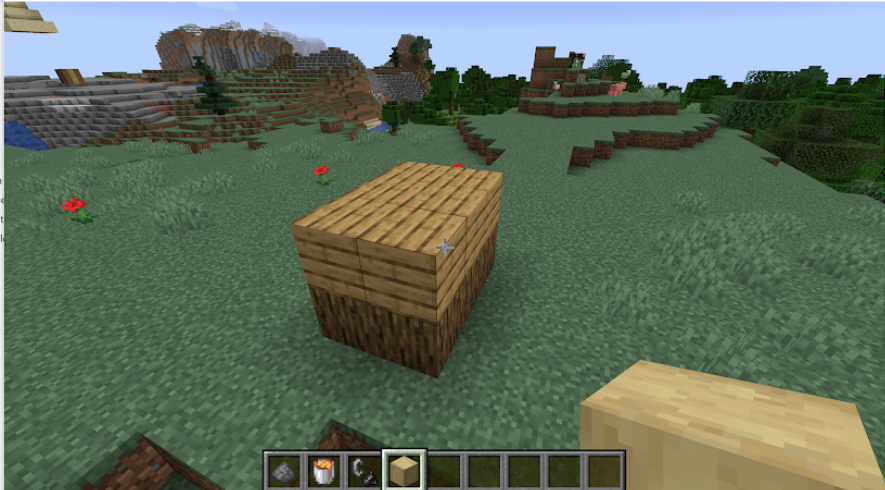
\includegraphics {example0.png}
\newline\newline
{\large Example 1:}\newline 

This example can be run with the following command from the minebuilder project directory:\newline
\textbf{dotnet run ../../examples/example-1.mc} \newline
Note: On Windows, make sure to change forward slashes to backlashes for proper pathing.

\begin{verbatim}
// defines a variable, storing the given blueprint in "struct."
// struct is a wooden box in this example
define struct as
{
    wWw
    WWW
    wWw
    -
    wWw
    WWW
    wWw
    -
    wWw
    WWW
    wWw
    -
}

// builds the defined structure at the given coordinates in Minecraft.
build struct (32,103,3012)
end
\end{verbatim}
The expected output is the following:
\begin{verbatim}
Program successfully executed. Please check Minecraft to see results!
Additionally, check mine.py for the Python interpretation of your source code.
\end{verbatim}
In Minecraft:\newline
\newline
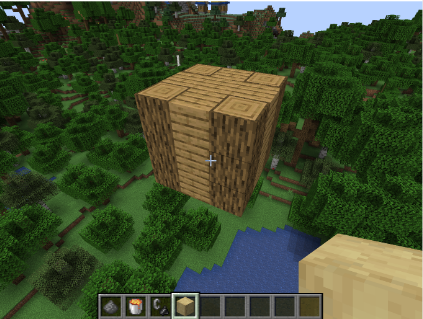
\includegraphics {example1.png}
\newline\newline
{\large Example 2:}\newline 

This example can be run with the following command from the minebuilder project directory:\newline
\textbf{dotnet run ../../examples/example-2.mc} \newline
Note: On Windows, make sure to change forward slashes to backlashes for proper pathing.

\begin{verbatim}
define pyramid as
{
    //load the blueprint for a pyramid
    load pyramid.mpb
}

// builds the defined structure at the given coordinates in Minecraft.
build pyramid (-23,-30,-12)
end
\end{verbatim}
The expected output is the following:
\begin{verbatim}
Program successfully executed. Please check Minecraft to see results!
Additionally, check mine.py for the Python interpretation of your source code.
\end{verbatim}
In Minecraft:\newline
\newline
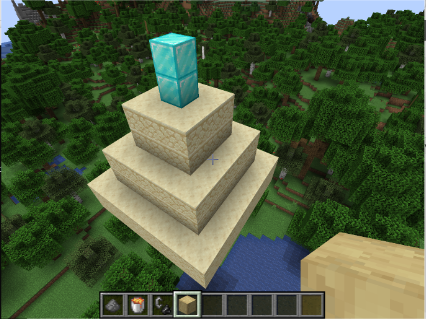
\includegraphics {example2.PNG}
\newline
\newpage
{\large Example 3:}\newline 

This example can be run with the following command from the minebuilder project directory:\newline
\textbf{dotnet run ../../examples/example-3.mc} \newline
Note: On Windows, make sure to change forward slashes to backlashes for proper pathing.

\begin{verbatim}
// defines a variable, storing the given blueprint in "boulder"
define boulder as
{
    .C.
    CCC
    .C.
    -
    CCC
    CCC
    CCC
    -
    .C.
    CCC
    .C.
    -
}

// defines a variable, storing the given blueprint in "house"
define house as
{
    //load the blueprint for a house
    load house.mpb
}

// repeatedly builds the given structures at the given Minecraft coordinates 
// specifies the distance apart, and the direction of subsequent repetitions

repeat boulder starting at (100,80,-400) for 20 times, 3 apart in y direction
repeat house starting at (0,0,0) for 20 times, 10 apart in x direction
end
\end{verbatim}
The expected output is the following:
\begin{verbatim}
Program successfully executed. Please check Minecraft to see results!
Additionally, check mine.py for the Python interpretation of your source code.
\end{verbatim}
In Minecraft:\newline
\newline
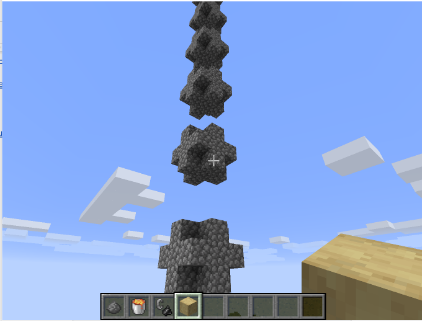
\includegraphics {example3.PNG}
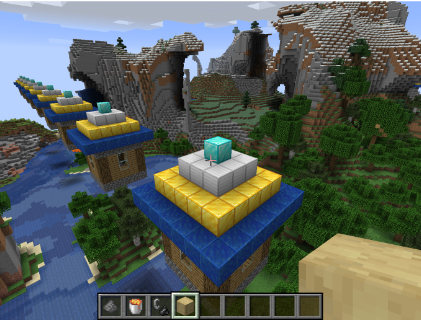
\includegraphics {example3-2.PNG}
\newline
\section{Language Concepts}
In MineBuilder, a user defines blueprints of Minecraft structures that are later built using \textbf{build} or \textbf{repeat} commands. Blueprints are 3D structures, represented as a sequence of 2D slices made up of lines of specific ASCII characters corresponding to blocks in Minecraft. These horizontal slices are delimited by "-". Using these blueprints, a user can build or repeat any structure to their heart's desire in the world of Minecraft. \newline 

In order to communicate with the game, programs interface with Python and Spigot Minecraft servers running on the machine. Therefore, in order to run these types of programs, you will need to install the Minecraft Python API, and make sure you are running a properly configured Spigot Minecraft server. For more information on how to set up the Minecraft Python API, visit this \underline {\href{https://medium.com/@kidargueta/learn-python-with-minecraft-part-1-setting-up-the-environment-fa0c7f9e3ca6}{tutorial.}}

\section{Syntax}
\begin{verbatim}
WHERE + = one or more
WHERE * = zero or more

<program>       ::=  <command>+
<command>       ::=  <define><nl>+
                     | <build><nl>+
                     | <repeat><nl>+
                     | <end>
<define>        ::= define <name> as<nl><blueprint>
<build>         ::= build <name> at <coords>
<repeat>        ::= repeat <name> starting at <coords> for <num> times, 
                     <num> apart in <dir> direction
<end>           ::= end
<name>          ::= <character>+
<character>     ::=  any in {a..z,A ...Z}
                    | <num>
                    | <hyphen>
                    | _ 
<hyphen>        ::= -
<blueprint>     ::=   {
                         <slice>+
                      }
                    | {
                        load <filename>
                      }
<dir>           ::= any in {x,y,z,X,Y,Z}
<filename>      ::= <character>+ .mpb
<slice>         ::= <line>+ <nl> <hyphen>
<line>          ::= <block_chars>+ <nl>
<block_chars>   ::= any in {block character set}
<coords>        ::= (<num>,<num>,<num>)
<num>           ::= any in Integers
<nl>            ::= \n
\end{verbatim}

\newpage
\section{Semantics}
1. The \textbf{define} statement, which defines a name as a certain blueprint. Its usage is as either of the following:

\begin{multicols}{2}
\begin{verbatim}
define name as
{
    load example.mpb
}


define name2 as
{
    www
    WWW
    -
}
\end{verbatim}
\end{multicols}

Both invocations adds the name-blueprint tuple to the global environment. The left loads example.mpb, a file, and associates it with name, while the right simply associates the given blueprint with name2. In the Abstract Syntax Tree, they are stored as a \textbf{Define} of (string * Blueprint) \newline


2. The \textbf{build} statement, which builds the blueprint associated with a name at the given coordinates in Minecraft. Its usage is the following:

\begin{verbatim}
build name at (0,100,200)
build name2 at (-2,-2,-2) 
\end{verbatim}

The \textbf{Build} command connects with the Minecraft client and builds the blueprint at the given coordinates. The first builds name at (0,100,200), and the second builds name2 at (-2,-2,-2). In the AST, they are stored as a \textbf{Build} of (string * Coords) \newline

3. The \textbf{repeat} statement, which repeats the blueprint associated with a name at the given coordinates in Minecraft for a given number of times, with a given distance, in the given direction. Its usage is the following:

\begin{verbatim}
repeat name starting at (0,100,200) for 20 times, 3 apart in y direction
repeat name2 starting at (-2,-2,-2) for 5 times, 10 apart in x direction
\end{verbatim}

The \textbf{Repeat} command connects with the Minecraft client and repeats the blueprint, starting at the given coordinates, and continuing for the given number of times in the given direction, with the given distance separating each instance. The distance is measured from the widest points of the blueprint in the given direction. The first repeats name for 20 times, 3 apart in the Y direction starting at (0,100,200). The second repeats name2 for 5 times, 10 apart in the X direction starting at (-2,-2,-2) In the AST, they are stored as a \textbf{Repeat} of (string * Coords * int * int * char) \newline

4. The \textbf{end} statement, which signals that the program is over and tells the interpreter to build and run the Python file. Its usage is the following:

\begin{verbatim}
end
\end{verbatim}

The \textbf{End} command is what signals to the interpreter that the program is done, and actually writes the output of the previous build and repeat commands to Python.  Then, it will run the Python script to build the delineated structures in the game, and close execution.  In the AST, they are stored as an \textbf{End}. \newline

Others. In order to use the above commands, the following two data types are used:

1. The three data types that make up the \textbf{Blueprint} data type are of the structure:

\begin{verbatim}
Blueprint of Slice list
Slice of Line list
Line of char list
\end{verbatim}

All together, these three represent the three dimensions of the Blueprint. Each Blueprint represents the 3D encoding of the given structure. Each Slice represents a 2D X-Z slice of the given structure. Each Line represents a 1D x-dimension block line of the given structure, encoded as characters. \newline 

2. The \textbf{Coords} data structure is simply a 3-tuple of three integers.  

\newpage
\section{Remaining Work}
Much of the desired functionality of our language has already been implemented, as users can define blueprints, build them, and build them repeatedly. \newline

To that end, the following are some \emph{stretch goals} we would have liked to implement given infinite time and resources:

1. A way to combine blueprints in an intuitive way, such as defining them in terms of each other (e.g. a house defined as a combination of a special roof, walls, floor, and ceiling) \newline

2. A way to alter the dimensions of the blueprints (such that they could be built using any direction of 2D slices including X-Y and Y-Z) \newline

3. A refactoring that would eliminate the need to use the Python API - this is the most difficult of the three, as it would involve creating a user mod for Minecraft to directly interface with our program. \newline

4. If the following refactoring was completed, an interactive REPL that built structures in realtime, allowing instant feedback and troubleshooting. \newline

% DO NOT DELETE ANYTHING BELOW THIS LINE
\end{document}
